\documentclass[journal]{IEEEtran}

\usepackage{blindtext}
\usepackage{graphicx}
\usepackage{hyperref}
\usepackage{listings}

\usepackage{tikz}
\usetikzlibrary{arrows,shapes,positioning}
\usetikzlibrary{calc,decorations.markings}

\tikzstyle{block} = [
  rectangle, draw, rounded corners, text centered, text width =
  7em, minimum height = 2em
]
\tikzstyle{rblock} = [
  rectangle, draw, text centered, text width =
  7em, minimum height = 2em
]
\tikzstyle{dottedblock} = [
  rectangle, draw, rounded corners, text centered, text width =
  7em, minimum height = 2em,dashed
]
\tikzstyle{line} = [draw, -latex']

\usepackage[backend=bibtex]{biblatex}
\addbibresource{/Users/brucecollie/Documents/Uni/Academic/zotero.bib}

\ifCLASSINFOpdf
  % \usepackage[pdftex]{graphicx}
  % declare the path(s) where your graphic files are
  % \graphicspath{{../pdf/}{../jpeg/}}
  % and their extensions so you won't have to specify these with
  % every instance of \includegraphics
  % \DeclareGraphicsExtensions{.pdf,.jpeg,.png}
\else
  % or other class option (dvipsone, dvipdf, if not using dvips). graphicx
  % will default to the driver specified in the system graphics.cfg if no
  % driver is specified.
  % \usepackage[dvips]{graphicx}
  % declare the path(s) where your graphic files are
  % \graphicspath{{../eps/}}
  % and their extensions so you won't have to specify these with
  % every instance of \includegraphics
  % \DeclareGraphicsExtensions{.eps}
\fi

\hyphenation{op-tical net-works semi-conduc-tor}

\begin{document}

\lstset{language=C}
\lstset{
  basicstyle=\footnotesize\ttfamily,
  showstringspaces=false
}

\title{Dynamic Discovery of Parallelisable Code}
\author{Bruce Collie, Trinity Hall}

\markboth{Modern Compiler Design, Part III Computer Science 2016-17}{}

\maketitle

\begin{abstract}

  The automatic discovery of parallelism in programs has been a goal of compiler
  engineers for many years. However, many traditional static analysis techniques
  fail to do so effectively. In this report I describe a dynamic approach to
  discovering potentially parallelisable code in C programs using an iterative
  approach to compilation. I provide a framework for integrating iterative
  compilation into a project, and show how this approach can be used to refine
  the structure of a C program based on dynamic analysis of the program's
  execution. Further to this, I discuss the limitations of my approach and how
  future work could provide stronger analyses and a more complex evaluation
  framework for executions. Finally, I give demonstrations of the tool being
  used on both simple example programs written for this purpose and a larger
  corpus of open source code, along with an evaluation of the successes and
  failures of this type of analysis.

\end{abstract}

\begin{IEEEkeywords}
auto-parallelisation, optimisation, dynamic analysis
\end{IEEEkeywords}

\IEEEpeerreviewmaketitle

\section{Introduction} \label{sec:intro}

An increasingly prevalent trend in computer hardware is that of parallelism.
More than ever, improvements in single-threaded performance are slow in
comparison to increased parallelism (in many different forms, such as GPGPU
computation or hyper-threaded CPU cores). However, writing concurrent code that
is both performant and correct remains an open problem in software engineering.
The inherent difficulty in this task arises for a number of different
reasons---cognitive overhead caused by increased complexity in the programming
model, difficulty in debugging nondeterministic executions, and unintuitive
performance characteristics. It is for these reasons that the goal of having
parallelism in programs be automatically detected and exploited is attractive.
Being able to abstract away as many of the problems of writing parallel code as
possible means that programmers will be able to work more effectively using
modern hardware and software features.

The automatic discovery of parallel structure in code is made far more difficult
by the unstructured way in which programs are usually written.  The intent of a
piece of code may not be easily determined from its textual representation,
especially in a language with little abstraction from the hardware such as C.
Some previous work aims to deliberately write programs such that they are
parallel by construction (for example, the language of ``Parallel Skeletons''
described by \textcite{gorlatch_parallel_2011} composes larger programs out of
parallel primitives). In some cases, these structured approaches are optimisable
for significant performance gains (an example of this is the machine-learning
approach taken by \textcite{collins_masif:_2013} to optimising parallel
skeletons).

However, these approaches are not broadly applicable to existing code.
\textcite{maleki_evaluation_2011} give an evaluation of auto-vectorising
implementations in mainstream C compilers, finding that almost all of the
available opportunities are not capitalised upon by the static analysis
techniques used.

In this report I describe an alternative method for discovering potentially
parallelisable code in C programs. \textcite{fursin_evaluating_2002} introduce
the idea of \emph{iterative compilation}, where a program is compiled in
multiple steps with feedback applied at each step to improve the program. I
present a basic implementation of the iterative compilation idiom that uses the
runtime behaviour of programs to provide feedback to successive compilations.
This implementation is then used (together with user feedback) to discover and
annotate possible source-level parallelism in a program. I evaluate the success
of this approach compared to a static analysis with similar goals.

\section{Dynamic Analysis} \label{sec:dynamic}

In this section I specify the dynamic analysis that will be performed on
programs, as well as the implementation of this analysis. I also compare the
analysis to a static version that aims to discover similar patterns in code.

\subsection{Specification} \label{ssec:spec}

\textcite{darlington_parallel_1995} describe a number of the primitive
``parallel skeletons'' that can be composed to implement a larger program.
Perhaps the simplest of these primitives is \texttt{map}, which simply performs
a given operation for every element of a collection (this could be a computation
and assignment to another array, or a call to a side-effecting function). In the
language of parallel skeletons, each operation must be independent of all the
others such that execution of the \texttt{map} is parallelisable (or more
accurately, that the result of the map is independent of the way in which its
subtasks are executed). The core of a simple \texttt{map} is given in
\autoref{lst:map}.

\begin{figure}[h]
  \centering
  \begin{lstlisting}
int f(int);

void map(int *in, int *out, size_t n) {
  for(size_t i = 0; i < n; i++) {
    in[i] = f(out[i]);
  }
}
  \end{lstlisting}
  \caption{Simple \texttt{map} operation written in C}
  \label{lst:map}
\end{figure}

The simplicity of the example in \autoref{lst:map} is somewhat deceptive. There
are many possible variations on the idea that may disguise the underlying intent
of the code (e.g.\ intermediate computations and function calls or control
flow). \autoref{lst:map-bad} gives an example in which the map structure is less
obvious. 

\begin{figure}[h]
  \centering
  \begin{lstlisting}
int f(int);

void map_complex(int *in, int *out, size_t n) {
  for(size_t i = 0; i < n; i++) {
    int value = in[i];

    if(f(value) > 0) {
      out[i] = 0
    } else {
      out[i] = f(value) + f(0);
    }
  }
}
  \end{lstlisting}
  \caption{More complex \texttt{map} operation that includes control flow}
  \label{lst:map-bad}
\end{figure}

The key property that both of these examples share is that (subject to
\texttt{f} being free of side effects), the order of loop execution is not
important to the behaviour of the loop as a whole. That is, the loop iterations
could be reordered while preserving behaviour.

This property motivates the dynamic analysis implemented as part of this
project---if the iterations in a loop can be reordered without changing the
program's behaviour, then there is a good chance that the loop can be
parallelised. It is worth noting that this analysis cannot identify
parallelisable loops with complete certainty. For example, if iterations share
state, then interleaving executions can cause behavioural changes not observable
only by reordering iterations in a sequential execution. This is one of the
fundamental trade-offs between static and dynamic analysis, and is discussed in
more depth in \autoref{sec:eval}.

\subsection{Implementation} \label{ssec:impl}

The primary goal of the dynamic analysis implemented in this project is to
identify loops that could potentially be parallelised, and subsequently to
reorder the iterations of these loops in an attempt to trigger changes in the
program's behaviour. If there are no such changes, then there is some evidence
that the loop could be parallelised (though as discussed previously, this
evidence is not conclusive).

\subsubsection{Clang Tooling}

Clang provides a rich set of libraries for analysing and modifying source code,
at both the textual and AST levels. In particular, the AST matchers framework
allows for predicates on the AST to be written that match nodes with a certain
structure. Components of these nodes can have names bound to them and analysed
as required. The implementation of the loop reordering component of the dynamic
analysis uses this framework to detect loop structures in the code that can
potentially be reordered, as well as the source rewriting support in Clang to
perform the modification of source files. 

\begin{figure}[h]
  \centering
  \begin{lstlisting}
unaryOperator(
  hasOperatorName("++"),
  hasUnaryOperand(ignoringParenImpCasts(
    declRefExpr(
      to(varDecl(hasType(isInteger())
    )
  )
)
  \end{lstlisting}
  \caption{AST matcher that matches an increment of an integer variable}
  \label{lst:astm}
\end{figure}

Idiomatically, Clang tools that analyse source code can either make changes in
place to the file or output a modified file to standard output. Because of this,
the loop reordering component simply replaces loops in a source file with a
reordered version. In \autoref{sec:iter}, a description of the tooling developed
to better integrate this into a traditional development workflow is given.

\subsubsection{Reordering Strategies}

There are many different ways in which a particular \texttt{for} loop could be
reordered. For example, iteration could be reversed, or all even iterations
could be executed first. Not every loop can be reordered in every possible
way---to work around this problem, I implemented several different
``strategies'' for reordering a loop:

\textbf{Reverse:} the loop iterates in reverse order. This strategy can be
applied to any conventionally structured \texttt{for} loop (that is, one that
has an initializer, upper bound and loop increment).

\textbf{Random:} if the loop initializer and upper bound are compile-time
constants, then loop iterations can be randomly ordered by unrolling the loop at
the source level (with an unrolled instance of the body for each loop
iteration).

\textbf{Odd-Even:} half of the iterations are executed first, then the other
half. This requires that the loop increment is exactly 1 (so that the two
reordered copies can each have an increment of 2).

Each of these strategies is implemented as a method that takes a Clang
\texttt{ForStmt} node together with some contextual information, then returns a
string representing the reordered loop. This string is then used as a direct
replacement for the detected loop.

The tool accepts a command line parameter specifying the reordering strategy to
be used on a source file. Each strategy specifies an AST matcher that detects
loops with the appropriate structure (for example, the odd-even matcher
specifies an increment of 1, and the random matcher specifies compile-time
constant initial and bound values).

\subsubsection{Experimentation}

Because the reordered loops are intended to be run experimentally (so as to
determine whether or not their reordering affects the behaviour of the program),
the tool only reorders a single loop at a time when it is run on a source file.
If more loops were reordered, it may become difficult to determine which
reordering caused a behavioural change. By default, the first detected loop for
a given strategy is reordered and all others are left unmodified.

To allow the tool to be used as part of an experimental process, the tool prints
the file name and source line on which the reordered loop was detected to
standard output.

\subsubsection{Summary}

To summarise, the initial component of the dynamic analysis method implemented
by this project is a command line utility that when passed the name of a source
file and a reordering strategy, will attempt to detect a reorderable loop in the
source file. If one is found, the reordering strategy is applied, modifying the
file in place. The source location of the reordered loop is printed to standard
output.

\begin{figure}[h] 
  \centering 
  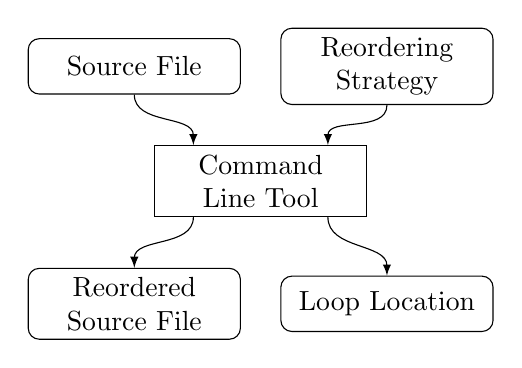
\begin{tikzpicture} 
    \node[block] (source) {Source File}; 
    \node[block, right=0.5cm of source] (strategy) {Reordering Strategy};
    \path (source) -- node[rblock, below=1 cm] (cli) {Command Line Tool} (strategy);
    \node[block, below=2.2cm of source] (re-source) {Reordered Source File};
    \node[block, right=0.5cm of re-source] (loc) {Loop Location};

    \path[-latex] (source.south) edge[out=270, in=90] ([xshift=5mm] cli.north west);
    \path[-latex] (strategy.south) edge[out=270, in=90] ([xshift=-5mm] cli.north east);
    \path[-latex] ([xshift=5mm] cli.south west) edge[out=270, in=90] (re-source.north);
    \path[-latex] ([xshift=-5mm] cli.south east) edge[out=270, in=90] (loc.north);
  \end{tikzpicture} 
  \caption{Data flow in the loop reordering component}
  \label{fig:tool}
\end{figure}


\subsection{Static Analysis}

As well as the dynamic analysis described in \autoref{ssec:impl}, I investigated
the implementation of a static method of performing a similar analysis. A
comparison of the two methods is given in \autoref{ssec:compare}. As with the
dynamic analysis described previously, the Clang AST matching framework was used
to match structures within the program's AST.

In order to statically detect loops that are structured as a \texttt{map}, I
wrote AST matchers that matched \texttt{for} loops with a particular structure.
The basic structural criteria for loops that could possibly be parallelised
were:

\begin{itemize}
  \item Must initialize a variable to a constant value in the loop initializer
    (with or without declaring it).
  \item Must check whether that variable is less than a constant value in the
    loop condition.
  \item Must increment the loop variable (pre- or postfix).
\end{itemize}

These criteria are in fact overly strict, but they characterise those loops that
iterate over a fixed range in increasing order. It is possible that a loop
intended to act as a \texttt{map} operation iterates in a different way, but in
the interests of keeping the AST matching code tractable, more complex matching
strategies were not used.

Once a loop with the correct iteration structure has been identified, its body
must be analysed separately to determine whether or not it performs a mapping
operation. Unfortunately, characterising an arbitrary AST fragment as having a
specific intent is not an easy problem---the AST matching idiom only allows for
exact (modulo ``implicit'' components such as casts or parentheses) matches to
be detected. As a result, each possible behaviour that a loop could have must
be encoded as an AST matcher. In addition, further analysis is likely to be
needed (for example, to ensure that the loop iteration structure is not altered
inside the loop body).

For these reasons, and as it was not the primary focus of this project, only a
limited set of loop body AST matchers and analyses were implemented:

\begin{itemize}
  \item Assignment to an element of an array, where the value being assigned is
    an expression that includes a reference to the loop iteration variable.
    Additionally, a check that the array is not assigned to by other code in the
    body.
  \item Check to ensure that neither the loop bound (if it is a variable) nor
    the loop iteration variable are assigned to.
\end{itemize}

\section{Iterative Compilation Framework} \label{sec:iter}

In this section I describe the framework I have implemented to integrate the
dynamic analysis described in \autoref{sec:dynamic} into a project written in C.

\subsection{Background}

A modern C compiler implements a multi-stage pipeline that transforms source
code into an executable format. \autoref{fig:pipeline-static} shows a simplified
version of this pipeline---source code is parsed into a tree structure, which is
then compiled into an intermediate representation, and finally lowered into
target code. Each stage of the pipeline is independent of the results of future
stages, and the data flow is unidirectional.

\begin{figure}[h] 
  \centering 
  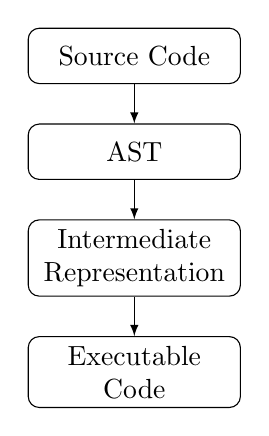
\begin{tikzpicture} 
    \node[block] (source) {Source Code}; 
    \node[block, below=0.5cm of source] (ast) {AST};
    \node[block, below=0.5cm of ast] (ir) {Intermediate Representation};
    \node[block, below=0.5cm of ir] (exe) {Executable Code};

    \draw[-latex] (source.south) -- node[above] {} (ast.north);
    \draw[-latex] (ast.south) -- node[above] {} (ir.north);
    \draw[-latex] (ir.south) -- node[above] {} (exe.north);
  \end{tikzpicture} 
  \caption{Traditional compiler pipeline (simplified)} 
  \label{fig:pipeline-static}
\end{figure}

In contrast, iterative compilation allows data to flow ``backwards'' through the
pipeline. Output from a stage can inform the action of a previous stage (on the
next compilation of the program), as shown in \autoref{fig:pipeline-dynamic}. In
the context of this project, the feedback takes the form of loop reorderings as
generated by the command line tool described previously.

\begin{figure}[h] 
  \centering 
  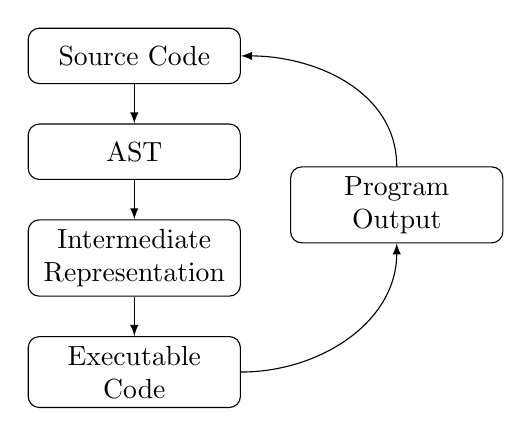
\begin{tikzpicture} 
    \node[block] (source) {Source Code}; 
    \node[block, below=0.5cm of source] (ast) {AST};
    \node[block, below=0.5cm of ast] (ir) {Intermediate Representation};
    \node[block, below=0.5cm of ir] (exe) {Executable Code};
    \path (ast.east) -- node (mid) {} (ir.east);
    \node[block, right=0.5cm of mid] (out) {Program Output};

    \draw[-latex] (source.south) -- node[above] {} (ast.north);
    \draw[-latex] (ast.south) -- node[above] {} (ir.north);
    \draw[-latex] (ir.south) -- node[above] {} (exe.north);
    \path[-latex] (exe.east) edge[out=0, in=270] node [left] {} (out.south);
    \path[-latex] (out.north) edge[out=90, in=0] node [left] {} (source.east);
  \end{tikzpicture} 
  \caption{Iterative compiler pipeline (simplified)} 
  \label{fig:pipeline-dynamic}
\end{figure}

Compilation using an iterative compiler is likely to take a far greater time
than compilation using a traditional compiler (as time to compile depends not
only on the static complexity of the program, but on the execution time as
well). \textcite{fursin_evaluating_2002} suggest that their iterative strategy
is well suited to an embedded environment, where long compile times are a
worthwhile tradeoff for increased program efficiency at runtime.

\subsection{Program Behaviour} \label{ssec:behaviour}

Implementing an experimental framework around the loop reordering tool described
previously requires a notion of what it means for a program's behaviour to
change. This is obviously a subtle idea that will differ greatly from program to
program. However, within the scope of this program, only a comparatively simple
definition of program is considered---I restrict the definition of program
behaviour to be the text that is printed to \emph{standard output} by the
program.

Even when only considering command line programs, this definition is likely to
miss some aspects of program behaviour. For example, return code, standard error
and network requests are not considered. Another consequence of this restricted
definition is that programs must be deterministic in their output for a given
input. If they are not, then there is no general way to determine whether a
change in behaviour is intended or caused by an incorrect loop reordering.

\subsection{Implementation}

In \autoref{ssec:impl}, I described the implementation of a command line tool
that detected and reordered loops in a C source file. In this section I describe
the implementation of the associated tooling that allows for that tool to be
integrated into an iterative compilation strategy. The simplest possible usage
of this tool is a manual one---a programmer would be able to use this tool to
compile multiple versions of their software and evaluate the results themself.
Indeed, in some cases this may be the most appropriate usage. However, in most
cases it is likely to be more useful to have the iterative compilation
integrated into a program's build process.

This integration takes the form of a collection of scripts and a Makefile that
wrap the reordering tool and implement the iterative compilation process. A
summary of the data flow through the iterative compiler is given in
\autoref{fig:hacks}.

\subsubsection{Reordering}

A wrapper script for the reordering tool was written to automatically generate
reordered source files given a list of reordering strategies at the command
line. This wrapper is also responsible for making copies of the original source
file so that changes are not destructive. The source location output from the
reordering tool is forwarded back onto standard output (if all strategies report
the same location).

\subsubsection{Makefile}

A standard Unix Makefile was chosen as the build tool for this part of the
project. The Makefile is broadly similar to a standard ``generic'' C Makefile
(allowing for compilation of \texttt{.c} files into \texttt{.o} files which are
then linked into an executable). However, it also specifies one source file in
the project as an ``experiment''. This file is passed to the reordering script
described above to generate several reordered versions. The application is then
compiled several times, each time with a differently reordered version of the
experimental source file.

\subsubsection{Macros}

The interface between the programmer and the iterative compilation process is
three C macros: \texttt{MAYBE\_PAR\_FOR}, \texttt{NO\_PAR\_FOR} and
\texttt{PAR\_FOR}. Each of these replaces the keyword \texttt{for} in a C
program, and indicate whether or not a loop can be parallelised. The default
definition for all three macros is the same: 

\begin{lstlisting}
#define *_PAR_FOR(x) for(x,0)
\end{lstlisting}

This definition preserves the loop behaviour if the program is recompiled with
annotations. The effect of \texttt{,0} is to change the AST of the loop so that
it is not detected by the reordering tool after it has been annotated (such that
another loop is detected next time round).

Eventually, the programmer should redefine \texttt{PAR\_FOR} so that the loop is
parallelised appropriately. For example, if OpenMP \cite{dagum_openmp:_1998}
was the parallelisation strategy chosen:

\begin{lstlisting}
#define PAR_FOR(x) _Pragma("omp parallel for") for(x)
\end{lstlisting}

\subsubsection{Annotation}

The annotation script takes a command line parameter (`y', `n' or `m'), a file
and a line number. It then replaces the keyword \texttt{for} with the
appropriate macro on that line in the file.

\subsubsection{Running}

Finally, the iterative feedback to the compilation process is automatically
generated by a runner script. Given a list of strategies and an executable name
(as generated by the Makefile described above), this script executes the
compiled executable for each strategy. The output of the unmodified executable
is stored. If any of the reordered executables produce different output, then
the experiment has shown that the loop in question cannot be parallelised. The
annotation script can then be called to add a macro in the correct place in the
source file.

\begin{figure}[h]
  \centering
  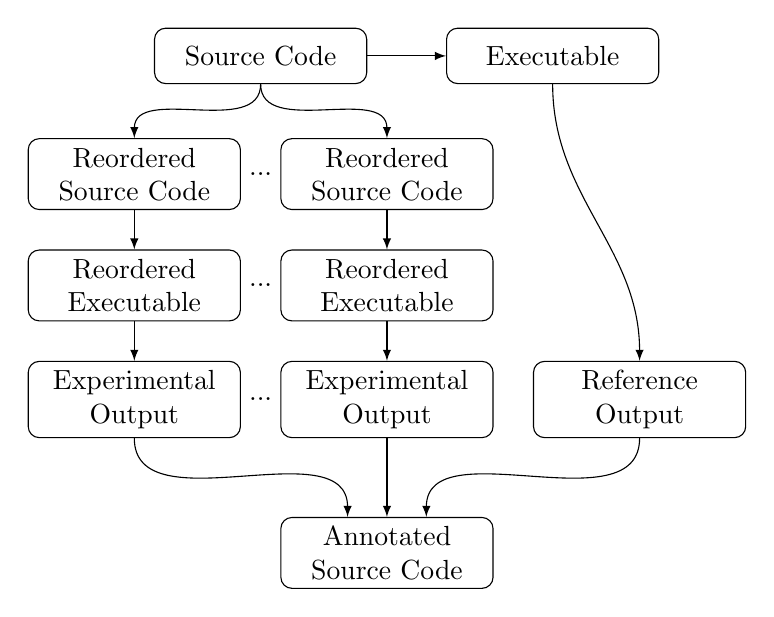
\begin{tikzpicture}
    \node[block] (re1) {Reordered Source Code};
    \node[block, right=0.5cm of re1] (re2) {Reordered Source Code};

    \node[block, below=0.5cm of re1] (exe1) {Reordered Executable};
    \node[block, below=0.5cm of re2] (exe2) {Reordered Executable};

    \path (re1) -- node (mid) {...} (re2);
    \path (exe1) -- node (mide) {...} (exe2);
    \node[block, above=1cm of mid] (source) {Source Code}; 
    \node[block, right=1cm of source] (exe) {Executable};

    \node[block, below=0.5cm of exe1] (out1) {Experimental Output};
    \node[block, right=0.5cm of out1] (out2) {Experimental Output};
    \node[block, right=0.5cm of out2] (out3) {Reference Output};
    \path (out1) -- node (mide) {...} (out2);

    \node[block, below=1cm of out2] (anno) {Annotated Source Code};

    \path[-latex] (source.south) edge[out=270, in=90] (re1.north);
    \path[-latex] (source.south) edge[out=270, in=90] (re2.north);
    \draw[-latex] (re1.south) -- (exe1.north);
    \draw[-latex] (re2.south) -- (exe2.north);
    \draw[-latex] (source.east) -- (exe.west);
    \draw[-latex] (exe1.south) -- (out1.north);
    \draw[-latex] (exe2.south) -- (out2.north);
    \path[-latex] (exe.south) edge[out=270, in=90] (out3.north);

    \path[-latex] (out1.south) edge[out=270, in=90] ([xshift=-5mm] anno.north);
    \draw[-latex] (out2.south) -- (anno.north);
    \path[-latex] (out3.south) edge[out=270, in=90] ([xshift=5mm] anno.north);
  \end{tikzpicture}
  \caption{Data flow through one step of the iterative compiler tooling. The
    annotated source code produced at the end of this process can be used as the
  input to the next step.}
  \label{fig:hacks}
\end{figure}

\section{Evaluation} \label{sec:eval}

In this section I describe the methodology by which the project was evaluated. I
give the results of this evaluation, as well as a summary of ways in which the
project could be improved in future work.

\subsection{Strategy}

The framework was evaluated against both example code constructed solely for the
purposes of evaluation and a larger body of existing code. This body of existing
code was chosen to be the GNU Scientific Library (GSL) 2.2.1
\cite{gough_gnu_2009} for the following reasons:

\begin{itemize}
  \item There is a large amount of code available for analysis. The
    \texttt{cloc} utility \cite{_aldanial/cloc_????} reports a total of 204,189
    lines of C code (not including headers, blank lines or comments).
  \item The code is largely concerned with implementing numerical algorithms,
    and so is likely to contain loops that are potentially parallelisable.
\end{itemize}

Because the GSL is a large project with its own complex build system,
integrating the automated tools described in \autoref{sec:iter} was not
practical. Instead, my evaluation was performed manually by writing a test
harness that linked against the GSL, then manually rebuilding reordered versions
of the GSL library code being examined.

\subsection{Comparison with Static Analysis} \label{ssec:compare}

\subsection{Possible Improvements and Further Work}

There are several issues with the dynamic analysis and iterative compilation
framework implemented in this project. Here I give a brief summary of each,
along with an indication of how the the issue might be mitigated in future work.

\subsubsection{Difficult to Integrate}

Integrating the iterative feedback loop into a traditional compilation model is
not easy. Traditional build tools do not support a ``feedback loop'', and so
support for this project needs to be built separately, greatly increasing the
complexity of a project's build system. A more streamlined set of tools and
scripts would alleviate this problem to some extent.

\subsubsection{Slow}

\subsubsection{False Positives}

\subsubsection{Limited Applicability} The limited definition of program
behaviour given in \autoref{ssec:behaviour} means that the tool cannot be
applied usefully to software whose primary interactions are not textual in
nature. \textcite{layton_io_2010} suggests monitoring the system calls made by
the executing software in order to characterise its IO behaviour. This is a
natural extension to the standard output model used in this report, but is
operating-system dependent in nature. It would also be possible to write an
application-specific testing script (for example, a UI automation tool) to
report behavioural regressions. This approach would be the most likely to
identify differences, but is the least portable between programs.

\section{Conclusion}

In this report I have described the implementation of a system for performing
iterative compilation of a C program, with feedback from a dynamic analysis of
loop reorderings. I have shown that this strategy can be used to discover
sources of potential parallelism within an existing codebase, and can be
integrated into new or smaller projects with a greater degree of automation.
Additionally, I have given the results of applying this model to a large corpus
of numerical code. I have compared this dynamic system to a static analysis with
similar goals, and shown the advantages and disadvantages of each method.
Finally, I have given a summary of the future work that could be done on this
system in order to improve its usability.

\ifCLASSOPTIONcaptionsoff
  \newpage
\fi

\printbibliography

\end{document}
